\section{Performance evaluation}

In this section we are going to evaluate the designed prototypes of the fluxionnal execution model, and compare it to the performance of a classical Javascript services.
We compare the implementation through three distincts web services giving users the exact same answers.
\begin{itemize}
	\item[Basic] The first one is a basic web service. It doesn't use fluxions.
	\item[Fluxionnal-NoSetTimeout] The second one is a fluxionnal web service, but fluxions are chained without the possibilies of interleaving messages from network as it doesn't use \texttt{SetTimeout}.
	\item[Fluxionnal] The third one is a fluxionnal web service, but networks messages can be executed between each local fluxion messages execution. It uses the instruction \texttt{SetTimeout}.
\end{itemize}

On the implementation level, the third one uses \texttt{SetTimeout} while the second one doesn't.
This difference make the second one incapable to handle fluxions chains longer than the function call stack size limit.

With these three differents programs, we want to highlight the advantages and drawbacks of the fluxionnal execution model.

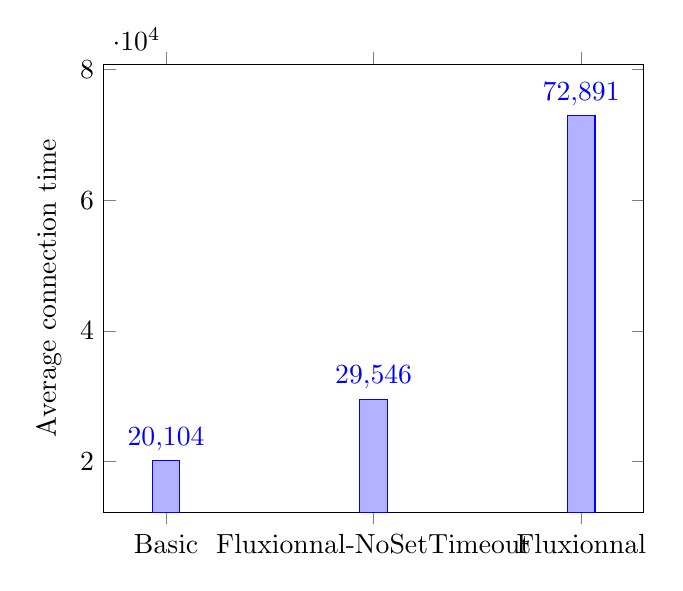
\begin{tikzpicture}
	\begin{axis} [
 		ybar,
 		enlargelimits=0.15, 
 		legend style={at={(0.5,-0.15)},anchor=north,legend columns=-1},
 		ylabel={Average connection time},
 		symbolic x coords={Basic,Fluxionnal-NoSetTimeout,Fluxionnal},
 		xtick=data,
 		nodes near coords,
 		nodes near coords align={vertical}
	]
		\addplot coordinates {(Basic,20104) (Fluxionnal-NoSetTimeout,29546) (Fluxionnal,72891)};
	\end{axis}
\end{tikzpicture}

We can see that the use of fluxions, from our implementation of the fluxionnal execution model increases the average response time of about 50\%, as the \textbf{Fluxionnal-NoSetTimeout} implementation aberage response time show from the \textbf{Basic} implementation.
However, the instruction \texttt{SetTimeout}, used in the original Fluxionnal execution model, increases the average response time of this implementation of about 360\%.